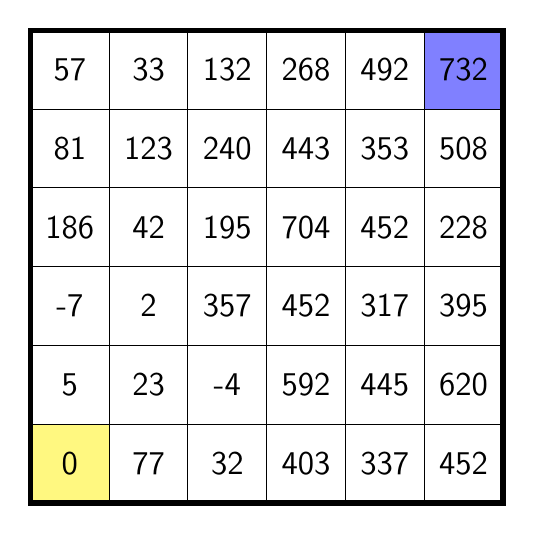
\begin{tikzpicture}
  \filldraw[color=yellow!50] (0,0)--(1,0)--(1,1)--(0,1)--cycle;
  \filldraw[color=blue!50] (5,5)--++(1,0)--++(0,1)--++(-1,0)--cycle;
  \def\drawNumber#1#2#3{\draw node at (#1+.5, #2+.5) {\large \textsf{#3}};}
  \drawNumber{0}{0}{0}
  \drawNumber{1}{0}{77}
  \drawNumber{2}{0}{32}
  \drawNumber{3}{0}{403}
  \drawNumber{4}{0}{337}
  \drawNumber{5}{0}{452}
  
  \drawNumber{0}{1}{5}
  \drawNumber{1}{1}{23}
  \drawNumber{2}{1}{-4}
  \drawNumber{3}{1}{592}
  \drawNumber{4}{1}{445}
  \drawNumber{5}{1}{620}
    
  \drawNumber{0}{2}{-7}
  \drawNumber{1}{2}{2}
  \drawNumber{2}{2}{357}
  \drawNumber{3}{2}{452}
  \drawNumber{4}{2}{317}
  \drawNumber{5}{2}{395}
  
  \drawNumber{0}{3}{186}
  \drawNumber{1}{3}{42}
  \drawNumber{2}{3}{195}
  \drawNumber{3}{3}{704}
  \drawNumber{4}{3}{452}
  \drawNumber{5}{3}{228}
  
  \drawNumber{0}{4}{81}
  \drawNumber{1}{4}{123}
  \drawNumber{2}{4}{240}
  \drawNumber{3}{4}{443}
  \drawNumber{4}{4}{353}
  \drawNumber{5}{4}{508}
  
  \drawNumber{0}{5}{57}
  \drawNumber{1}{5}{33}
  \drawNumber{2}{5}{132}
  \drawNumber{3}{5}{268}
  \drawNumber{4}{5}{492}
  \drawNumber{5}{5}{732}
  
    \draw[line width=2pt] (0,0)--(6,0)--(6,6)--(0,6)--cycle;
    \foreach \x in {1, ..., 5}{
      \draw (\x,0)--(\x,6);
    }
    \foreach \y in {1, ..., 5}{
      \draw (0,\y)--(6,\y);
    }
    \end{tikzpicture}
